\documentclass[sigconf]{acmart}
\usepackage{graphicx}   % Usually included by acmart
%% Remove if any conflict
\usepackage{subcaption} 
\usepackage{array} 
\newcolumntype{C}[1]{>{\centering\arraybackslash}p{#1}} 


%%
%% \BibTeX command to typeset BibTeX logo in the docs
\AtBeginDocument{%
  \providecommand\BibTeX{{%
    Bib\TeX}}}

% % % % % % % % % % % % % % % % % % % % % % % % % % % % % % % % % %
%
%            THE DEFINITIVE STUDENT PAPER SOLUTION
%
% This tells the template that the author retains all rights,
% which is perfect for a university project.
%
% % % % % % % % % % % % % % % % % % % % % % % % % % % % % % % % % %

% 1. Set the copyright type to 'rightsretained'.
\setcopyright{rightsretained}

% 2. Clear out all the specific ACM conference details so they don't appear.
%    This is still a good practice to ensure no defaults slip through.
\acmConference[]{}{}{}
\acmBooktitle{}
\acmPrice{}
\acmISBN{}
\acmDOI{}

% % % % % % % % % % % % % % % % % % % % % % % % % % % % % % % % % %
%             END OF CUSTOM COPYRIGHT BLOCK
% % % % % % % % % % % % % % % % % % % % % % % % % % % % % % % % % %



% These must come BEFORE \begin{document}
\settopmatter{printacmref=false}      % This is the one that removes the copyright block
\renewcommand\footnotetext{}          % This removes the footnote version of the copyright

%%
%% end of the preamble, start of the body of the document source.
\begin{document}

%%
%% The "title" command has an optional parameter,
%% allowing the author to define a "short title" to be used in page headers.
\title{{Bridging Theory and Practice: An Empirical Analysis and Optimization of the GRU-ODE-Bayes Model}}



\author{Gabriel Martins Silveirda de Oliveira}
\affiliation{%
  \institution{University of Brasília (UnB)}
  \city{Brasília}
  \country{Brazil}}
\email{daturasoldev@gmail.com}


%%
%% The abstract is a short summary of the work to be presented in the
%% article.
\begin{abstract}
Continuous-time models based on Neural Ordinary Differential Equations (NODEs) offer a theoretically 
elegant solution for modeling sporadically-observed time series, a common challenge in fields like healthcare. 
The GRU-ODE-Bayes model represents a state-of-the-art approach, combining the continuous dynamics of an ODE solver with 
discrete updates inspired by Gated Recurrent Units (GRUs). 
This paper presents a deep, practical investigation into the implementation and performance of the GRU-ODE-Bayes model on 
real-world physiological datasets. 
We detail a systematic journey of optimization, from robust data engineering to vectorized implementation, 
to make the model trainable. Our investigation reveals two surprising findings. 
First, due to the significant overhead of the adjoint-based ODE solver for sequential, short-interval tasks, 
a CPU-based training pipeline significantly outperforms its GPU counterpart. 
Second, and more critically, a simpler baseline model that omits the ODE component entirely is not only 
orders of magnitude faster to train (30 seconds vs. 1 hour per epoch) but also achieves substantially higher 
classification accuracy (97.78\% vs. 62\%). 
These results challenge the practical utility of the added complexity of the GRU-ODE-Bayes architecture for 
classification tasks on this type of data, highlighting a crucial gap between theoretical promise and empirical performance.
\end{abstract}


% %%
% %% Keywords. The author(s) should pick words that accurately describe
% %% the work being presented. Separate the keywords with commas.
\keywords{Neural Ordinary Differential Equations, 
GRU-ODE, Time Series, Adjoint Method, Performance Analysis, 
Computational Bottlenecks, Physiological Data}
%% A "teaser" image appears between the author and affiliation
%% information and the body of the document, and typically spans the
%% page.
\begin{teaserfigure}
  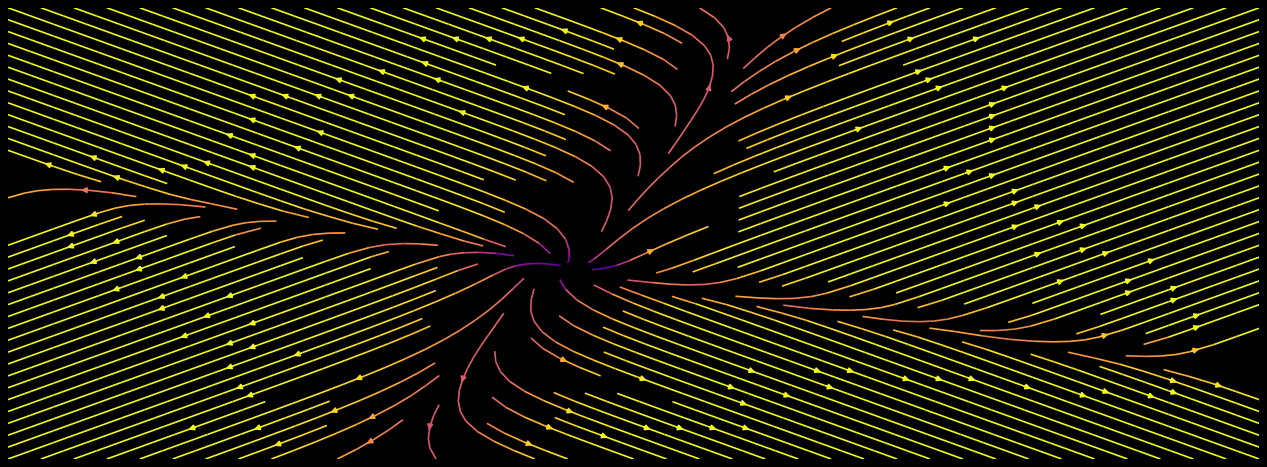
\includegraphics[width=\textwidth]{figures/teaser.png}
  \caption{A stream plot visualizing the vector field of a simple Neural ODE (NODE) cell. 
  The dynamics are defined by the equation $\frac{d \vec{y}}{dt} = \tanh(W \cdot \vec{y} + \vec{b})$ 
  with randomly initialized weights $W$ and biases $\vec{b}$. 
  The arrows illustrate the flow of the learned dynamical system before any training.}
  \Description{A 2D vector field visualization on a square plot. 
  The background is black, and the plot is filled small, curved, dark gradient arrows that form flowing lines. 
  The general flow moves from the bottom-left towards the top-right, 
  creating several swirls and points of convergence. 
  The overall visual texture resembles flowing water or wind patterns.}
  \label{fig:teaser}
\end{teaserfigure}


%%
%% This command processes the author and affiliation and title
%% information and builds the first part of the formatted document.
\maketitle

\fancyhead{}
%  \settopmatter{printacmref=false}
%  \renewcommand\footnotetext{} % Add this if the copyright notice still appears as a footnote

\section{Introduction}
\label{sec:introduction}

Modeling time series data with irregular and sporadic observations is a 
persistent challenge in machine learning, with critical applications in domains such as healthcare, 
finance, and climate science. 
Traditional Recurrent Neural Networks (RNNs) and their variants, 
like LSTMs and GRUs, are designed for sequences with fixed, 
regular time steps and struggle to naturally handle the continuous-time nature of 
real-world processes.

Neural Ordinary Differential Equations (NODEs) \cite{chen2019neuralordinarydifferentialequations} 
emerged as a powerful paradigm to address this limitation. 
By parameterizing the derivative of a hidden state with a neural network, NODEs learn a continuous-time dynamical 
system directly from data, allowing for evaluation at any point in time. 
The GRU-ODE-Bayes model \cite{debrouwer2019gruodebayescontinuousmodelingsporadicallyobserved} 
builds upon this foundation, proposing a sophisticated architecture that propagates a system's 
hidden state using an ODE solver between observations and applies discrete, 
GRU-inspired updates at the moments observations are available.

While theoretically elegant, the practical implementation and performance characteristics of such 
complex models are not widely documented. 
The journey from a research paper's mathematical formulation to a working, efficient implementation is often 
fraught with non-trivial engineering challenges. 
This paper presents a deep dive into this process for the GRU-ODE-Bayes model. 
We document our journey from a naive implementation to a robust, vectorized model, 
tackling issues of data imbalance and computational bottlenecks.

Our investigation, conducted on three real-world physiological time series datasets, yields surprising and critical insights.
We find that the computational overhead of the core ODE solver component makes the model train significantly 
faster on a CPU than on a high-end GPU. 
More importantly, we demonstrate that a simplified baseline model, which removes the continuous-time ODE dynamic 
entirely, is not only orders of magnitude faster but also dramatically more accurate for the task of arrhythmia classification. 
This work aims to bridge the gap between theory and practice, providing a critical analysis of the GRU-ODE-Bayes
model's effectiveness and highlighting the crucial need to benchmark complex architectures
against strong, simple baselines.

\section{Theoretical Background}
\label{sec:background}
To understand our work, we first review the two core concepts upon which the GRU-ODE-Bayes model is built.

\subsection{Neural Ordinary Differential Equations}

A Neural ODE models the continuous evolution of a hidden state vector
$\vec{z}(t)$ by defining its derivative with a neural network $f$:
\begin{equation}
    \frac{d\vec{z}(t)}{dt} = f(\vec{z}(t), t, \theta)
\end{equation}

Given an initial state $\vec{z}(t_0)$, the state at any later 
time $t_1$ can be found by integrating this differential equation:
\begin{equation}
    \vec{z}(t_1) = \vec{z}(t_0) + \int_{t_0}^{t_1} f(\vec{z}(t), t, \theta) dt
\end{equation}

This integration is performed by a numerical ODE solver. 
A key challenge is backpropagation through the solver. 
The adjoint sensitivity method \cite{chen2019neuralordinarydifferentialequations} 
provides a highly memory-efficient solution by solving a second, augmented ODE backwards 
in time to compute gradients. This allows for training with constant memory cost with respect to depth. 
A full derivation of the adjoint method is provided in 
Appendix~\ref{app:adjoint_method} and its generalization using a Hamiltonian formulation 
is in Appendix~\ref{app:hamiltonian_adjoint}.

\subsection{The GRU-ODE-Bayes Model}

The GRU-ODE-Bayes model \cite{debrouwer2019gruodebayescontinuousmodelingsporadicallyobserved} 
adapts the NODE framework for sporadically-observed time series. The core idea is twofold:
\begin{enumerate}
    \item \textbf{Between observations}, the hidden state $\vec{h}(t)$ evolves continuously 
    according to an ODE solver.
    \item \textbf{At an observation} $x_i$ at time $t_i$, the hidden state is updated using a 
    mechanism analogous to a GRU cell, incorporating the new information.
\end{enumerate}

The model also incorporates a Bayesian framework to quantify uncertainty, which involves minimizing the 
Evidence Lower Bound (ELBO).
This objective function includes a reconstruction loss and a KL-divergence term that regularizes the latent space. 
The derivation for the KL divergence between two Gaussian distributions, a key component of the ELBO, 
is provided in Appendix~\ref{app:kl_divergence}.


\section{Implementation and Optimization}
\label{sec:implementation}

We implemented the GRU-ODE-Bayes model in PyTorch, using the \texttt{torchdiffeq} 
library for its implementation of the adjoint method. 
Our goal was to classify cardiac conditions from physiological data.

\subsection{Datasets and Preprocessing}

We used three publicly available ECG databases: 
the BIDMC Congestive Heart Failure Database, 
the MIT-BIH Arrhythmia Database, 
and the MIT-BIH Normal Sinus Rhythm Database. 
The raw signals were preprocessed by:
\begin{enumerate}
    \item Filtering the signal to remove noise.
    \item Detecting R-peaks to identify heartbeats.
    \item Extracting QRS timings around each R-peak.
    \item Segmenting the long recordings into uniform, overlapping "chunks" of 512 observations 
    to create a dataset of manageable, equally-sized samples. 
    This step was critical to prevent GPU out-of-memory errors and stabilize training.
\end{enumerate}

\subsection{From Naive Loop to Vectorized Model}
A naive implementation of the GRU-ODE-Bayes model involves a Python \texttt{for} 
loop that iterates through each observation in a sequence, alternating between an ODE solve and a discrete update. 
This approach proved to be a major performance bottleneck due to high overhead from many small, sequential operations.

To overcome this, we re-architected the forward pass to be fully vectorized. 
Instead of looping, our final implementation performs:
\begin{enumerate}
    \item \textbf{A single, batched \texttt{odeint} call} to compute a 
    "base trajectory" for the hidden state over all required time points in the batch.
    \item \textbf{Vectorized tensor operations} (e.g., \texttt{gather}, \texttt{index\_add\_}) 
    to apply the effects of all discrete updates simultaneously to the base trajectory.
\end{enumerate}

This significantly reduced Python overhead and shifted the computation to a few large tensor operations, 
the ideal workload for modern deep learning frameworks.

\section{Experimental Results and Analysis}
\label{sec:results}

Our experiments were designed to evaluate both the performance and the predictive accuracy of our 
optimized GRU-ODE-Bayes model against a strong baseline.

\subsection{The GPU Performance Anomaly}

Despite our vectorization efforts, we observed a baffling performance characteristic: 
the model trained significantly slower on a high-end GPU than on a CPU.
\begin{itemize}
    \item \textbf{CPU Training Time (batch size 1):} $\sim$1 hour / epoch.
    \item \textbf{GPU Training Time (batch size 64):} $\sim$5 hours / epoch.
\end{itemize}

Systematic profiling revealed that the bottleneck was the \texttt{odeint\_adjoint} function itself. 
For this model's specific workload—solving many short ODE segments back-to-back—the fixed overhead of 
launching CUDA kernels and managing the adjoint state on the GPU dominated the actual computation. 
The CPU, with its lower call overhead for sequential tasks, proved more efficient for this particular operational pattern.

\subsection{Model Accuracy and Baseline Comparison}

The most critical part of our analysis was comparing the full GRU-ODE-Bayes model against 
a simple but powerful baseline. 
This baseline uses the exact same architecture but \textbf{removes the ODE solver}, 
replacing it with a simple identity function that carries the last hidden state forward. 
The results were stark, as shown in Table~\ref{tab:results}.

\begin{table}[h]
  \centering
  \caption{Performance and Accuracy Comparison.}
  \label{tab:results}
  \begin{tabular}{l c c}
    \toprule
    \textbf{Metric} & \textbf{GRU-ODE-Bayes} & \textbf{Baseline (No ODE)} \\
    \midrule
    Validation Accuracy & 62.0\% & \textbf{97.78\%} \\
    Training Time / Epoch & $\sim$1 hour (CPU) & $\sim$30 seconds \\
    \bottomrule
  \end{tabular}
\end{table}

The complex, theoretically-motivated GRU-ODE-Bayes model was not only 120 times slower but also drastically 
less accurate than the simple baseline. 
The continuous dynamics modeled by the ODE solver did not provide a useful inductive bias for this classification task; 
instead, it appears to have hindered learning, possibly by introducing numerical instability or an overly complex loss landscape.

\subsection{A Successful Application: Learning Dynamical Systems}

To isolate and demonstrate the power of the NODE concept for its intended purpose, we conducted a 
supplementary experiment on a classic dynamical systems problem: 
learning the dynamics of the Lotka-Volterra (prey-predator) model. 
Here, the task is not classification, but to learn the underlying vector field from sparse trajectory data.

We first compare the ground truth dynamics to the output of a standard Multi-Layer Perceptron (MLP) with a similar number of parameters. 
As shown in Figure~\ref{fig:lv_true_vs_mlp}, the standard MLP is unable to learn the rotational structure of the system,
demonstrating its lack of an appropriate inductive bias for this task.

\begin{figure}[h!]
  \centering
  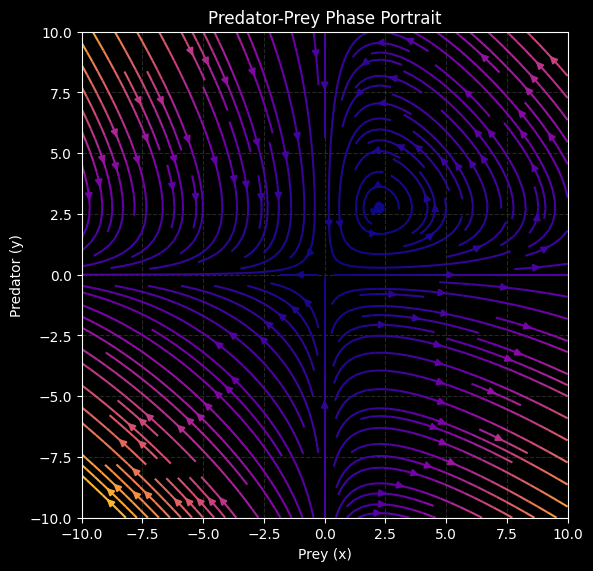
\includegraphics[width=0.8\linewidth]{figures/lv_true.png}
  \caption{The ground truth vector field of the Lotka-Volterra dynamical system, 
  showing its characteristic stable cycle.}
  \label{fig:lv_true_vs_mlp}
  \Description{A phase portrait plot showing the true spiral dynamics of the Lotka-Volterra system. 
  The vector field flows in a counter-clockwise spiral pattern.}
\end{figure}

\begin{figure}[h!]
  \centering
  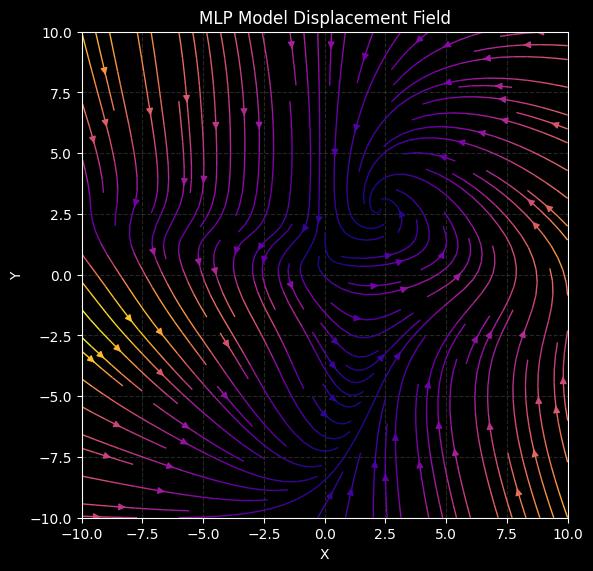
\includegraphics[width=0.8\linewidth]{figures/lv_mlp.png}
  \caption{The vector field learned by a standard MLP. 
  It fails to capture the rotational dynamics of the true system.}
  \label{fig:lv_mlp}
  \Description{A phase portrait plot from a standard MLP, 
  showing a distorted, non-rotational vector field.}
\end{figure}

Next, we evaluate two NODE-based models, differing only in their activation function. 
The results in Figures~\ref{fig:lv_tanh} and \ref{fig:lv_relu} are striking. 
The Tanh-based NODE captures a distorted sense of rotation but fails to accurately model the system. 
In contrast, the ReLU-based NODE almost perfectly reconstructs the vector field. 
This result confirms that NODEs possess a powerful inductive bias for learning continuous vector 
fields, but their success is highly dependent on both the problem domain and key architectural choices.

\begin{figure}[h!]
  \centering
  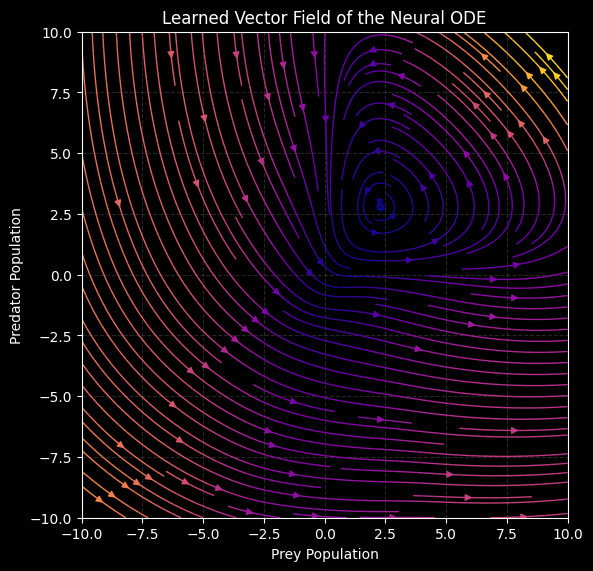
\includegraphics[width=0.8\linewidth]{figures/lv_tanh.png}
  \caption{The learned vector field from a NODE with a Tanh activation function. 
  The dynamics are distorted and inaccurate.}
  \label{fig:lv_tanh}
  \Description{A phase portrait plot from a Tanh-based NODE, showing a distorted spiral pattern.}
\end{figure}

\begin{figure}[h!]
  \centering
  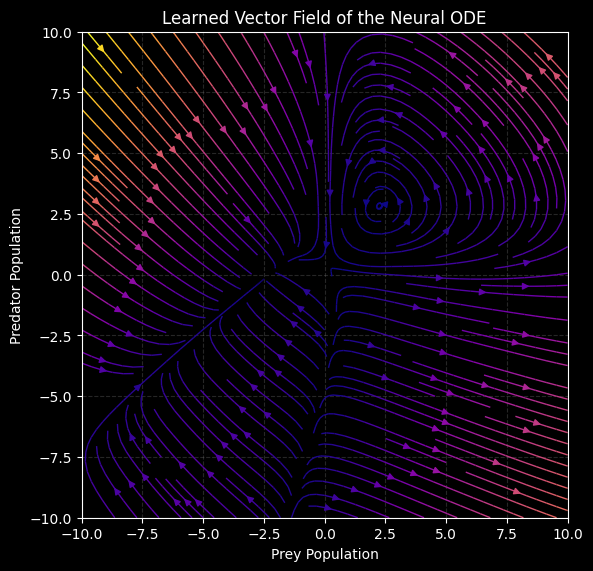
\includegraphics[width=0.8\linewidth]{figures/lv_relu.png}
  \caption{The learned vector field from a NODE with a ReLU activation function. 
  The model accurately reconstructs the true dynamics.}
  \label{fig:lv_relu}
  \Description{A phase portrait plot from a ReLU-based NODE, showing nearly perfect 
  spiral patterns identical to the ground truth.}
\end{figure}

\section{Discussion}
\label{sec:discussion}

Our findings present a cautionary tale about the application of complex models. 
The GRU-ODE-Bayes architecture, while theoretically compelling, failed to deliver on its promise for the practical 
task of arrhythmia classification on our datasets. 
The significant computational overhead and inferior performance compared to a simple baseline suggest that the 
model's core assumption—that modeling the continuous dynamics between heartbeats is beneficial—does not hold 
true for this problem. 
The classification task may depend more on the sequence of discrete QRS events rather 
than the subtle continuous evolution between them.

The performance anomaly where a CPU outperforms a GPU also serves as a critical reminder that hardware acceleration 
is not a universal solution. 
The nature of the computational workload is paramount, and algorithms involving many small, 
sequential steps may not benefit from a GPU's massively parallel architecture.

\section{Conclusion}
\label{sec:conclusion}

In this paper, we documented the implementation, optimization, and critical evaluation of the GRU-ODE-Bayes model. 
Through a rigorous process, we successfully trained the model on real-world physiological data, but discovered that its 
complexity was its downfall. 
A simpler baseline without the continuous-time ODE component was vastly superior in both speed and accuracy. 
Our work underscores the importance of empirical validation and the principle of Occam's razor in machine learning:
a simpler model that performs better is the better model. 
While Neural ODEs remain a powerful tool, particularly for learning physical dynamics, 
their application requires careful consideration of the problem's nature and a thorough 
comparison against strong, simpler baselines.


%% The acknowledgments section is defined using the "acks" environment
%% (and NOT an unnumbered section). This ensures the proper
%% identification of the section in the article metadata, and the
%% consistent spelling of the heading.
\begin{acks}
To Robert, for the bagels and explaining CMYK and color spaces.
\end{acks}

%%
%% The next two lines define the bibliography style to be used, and
%% the bibliography file.
\bibliographystyle{ACM-Reference-Format}
\bibliography{bib/references}


%%
%% If your work has an appendix, this is the place to put it.
\appendix

\section{Derivation of the Adjoint Method for Neural ODEs}
\label{app:adjoint_method}

\textit{This appendix provides a detailed derivation of the adjoint method as presented in Appendix B of the paper 
\cite{chen2019neuralordinarydifferentialequations}. 
The derivation here is presented in a more intuitive manner, aiming to deduce the result from 
first principles rather than starting with the definition of the adjoint state.}

\subsection{Context}

In a standard Recurrent Neural Network (RNN), a sequence of hidden states is generated, 
where each state carries information to the next:
\begin{equation}
    \vec{h}_{t+1} = \vec{h}_t + f(\vec{h}_t, \theta_t)
\end{equation}

The Neural Ordinary Differential Equation (NODE) model extends this concept to the continuous-time domain. 
As the time steps approach zero, the sequence of hidden states can be modeled as a continuous trajectory,
$\vec{z}(t)$, governed by an ordinary differential equation (ODE):
\begin{equation}
    \frac{d\vec{z}(t)}{dt} = \dot{\vec{z}} = f(\vec{z}(t), \theta, t)
    \label{eq:node_dynamics}
\end{equation}

We wish to find the gradient of a loss function $L$ with respect to the parameters $\theta$. 
Typically, $L$ depends directly only on the state at the final time, $L(\vec{z}(t_1))$. 
To find this gradient, we use the method of Lagrange multipliers to construct a new functional, $\mathcal{J}$, 
which incorporates the dynamic constraint of the ODE.

\begin{equation}
    \mathcal{J}(\vec{z}, \vec{\lambda}, \theta) =
    L(\vec{z}(t_1)) +
    \int_{t_0}^{t_1} \vec{\lambda}^{T}(t)
    \left[
    f(\vec{z}(t), \theta, t) - \dot{\vec{z}}(t)
    \right]
    \ dt
    \label{eq:adjoint_functional}
\end{equation}

By construction, the value of $\mathcal{J}$ is identical to $L$ whenever the dynamic constraint is satisfied. 
We analyze the first variation of $\mathcal{J}$, denoted $\delta\mathcal{J}$, by considering the contributions from each of its arguments:
\begin{equation}
    \delta \mathcal{J} =
    \frac{\delta \mathcal{J}}{\delta \vec{z}}\ \delta \vec{z} +
    \frac{\delta \mathcal{J}}{\delta \theta}\ \delta \theta +
    \frac{\delta \mathcal{J}}{\delta \vec{\lambda}}\ \delta \vec{\lambda}
\end{equation}

\subsection{First Variation of the Functional}

\subsubsection{Variation with Respect to $\vec{\lambda}$}

Setting the variation with respect to the Lagrange multiplier $\vec{\lambda}$ to zero recovers the original dynamic constraint:
\begin{equation}
    \frac{\delta \mathcal{J}}{\delta \vec{\lambda}} = f(\vec{z}, \theta, t) - \dot{\vec{z}} = 0 \quad \implies \quad \dot{\vec{z}} = f(\vec{z}, \theta, t)
\end{equation}

\subsubsection{Variation with Respect to $\theta$}

The contribution from the explicit dependence on the parameter $\theta$ is:
\begin{equation}
    \frac{\delta \mathcal{J}}{\delta \theta}\ \delta \theta =
    \int_{t_0}^{t_1} \vec{\lambda}^{T}(t)\
        \frac{\partial f}{\partial \theta}\ \delta \theta\ dt
\end{equation}

\subsubsection{Variation with Respect to $\vec{z}$}

The variation of $\mathcal{J}$ with respect to the trajectory $\vec{z}(t)$ is:
\begin{equation}
    \frac{\delta \mathcal{J}}{\delta \vec{z}}\ \delta \vec{z} =
    \frac{\partial L}{\partial \vec{z}(t_1)}\ \delta \vec{z}(t_1) +
    \int_{t_0}^{t_1} \vec{\lambda}^{T}(t)\left[
        \frac{\partial f}{\partial \vec{z}}
        \ \delta \vec{z} - \delta \dot{\vec{z}}\
    \right]\ dt
\end{equation}

We apply integration by parts to the term containing $\delta \dot{\vec{z}}$:
\begin{equation}
    -\int_{t_0}^{t_1} \vec{\lambda}^T \delta \dot{\vec{z}} \ dt =
    \int_{t_0}^{t_1} \dot{\vec{\lambda}}^T \delta\vec{z} \ dt -
    \left[\ \vec{\lambda}^T \delta\vec{z}\ \right]_{t_0}^{t_1}
\end{equation}

Substituting this back and rearranging terms yields:
\begin{equation}
    \begin{split}
        \frac{\delta \mathcal{J}}{\delta \vec{z}}\ \delta \vec{z} =
        & \left(
            \frac{\partial L}{\partial \vec{z}(t_1)} - \vec{\lambda}^T(t_1)
        \right) \delta\vec{z}(t_1) \\
        & + \vec{\lambda}^T(t_0)\ \delta\vec{z}(t_0) +
        \int_{t_0}^{t_1} \left[
            \vec{\lambda}^{T}\ \frac{\partial f}{\partial \vec{z}} +
            \dot{\vec{\lambda}}^{T}\
        \right]\delta \vec{z} \ dt
    \end{split}
\end{equation}

Since the initial condition $\vec{z}(t_0)$ is fixed, its variation $\delta\vec{z}(t_0)$ is zero. 
To nullify the remaining arbitrary variations, 
we strategically define the \textbf{adjoint state} $\vec{\lambda}(t)$ by enforcing two conditions:
\begin{enumerate}
    \item \textbf{Boundary Condition at Final Time ($t_1$):}
    \begin{equation}
        \vec{\lambda}^T(t_1) = \frac{\partial L}{\partial \vec{z}(t_1)}
        \label{eq:adjoint_bvp}
    \end{equation}
    \item \textbf{Differential Equation of the Adjoint State:}
    \begin{equation}
        \dot{\vec{\lambda}}^{T}(t) = - \vec{\lambda}^{T}(t)\ \frac{\partial f}{\partial \vec{z}}
        \label{eq:adjoint_dynamics}
    \end{equation}
\end{enumerate}

By imposing these conditions, the entire variation with respect to $\vec{z}$ vanishes.

\subsection{Final Result}
With the variations with respect to $\vec{z}$ and $\vec{\lambda}$ being zero, the total variation 
$\delta L = \delta \mathcal{J}$ simplifies to only the explicit contribution from $\theta$:
\begin{equation}
    \frac{d L}{d \theta}\ \delta \theta =
    \int_{t_0}^{t_1} \vec{\lambda}^{T}(t)\
        \frac{\partial f}{\partial \theta}\ \delta \theta\ dt
\end{equation}

This gives the final expression for the gradient of the loss function:
\begin{equation}
    \frac{d L}{d \theta} =
    \int_{t_0}^{t_1} \vec{\lambda}^{T}(t)\
        \frac{\partial f}{\partial \theta}\ dt
    \label{eq:adjoint_grad}
\end{equation}

\section{Generalized Adjoint Method via Hamiltonian Formalism}
\label{app:hamiltonian_adjoint}

Building upon the previous derivation, we can generalize the adjoint method for more complex
models by employing a Hamiltonian framework, inspired by optimal control theory. 
This is particularly useful for models like GRU-ODE-Bayes that may include a running loss term.

We define a total loss functional $T_L$ that includes both a final loss and an integrated loss over the trajectory:
\begin{equation}
    T_L(\vec{q}_n, \theta, t_1, t_0) = L(\vec{q}_n(t_1)) + \int_{t_0}^{t_1} \mathcal{L}(\vec{q}_n(t), \theta, t)\ dt
    \label{eq:total_loss}
\end{equation}

The system is subject to the dynamic constraint $\dot{\vec{q}}_n(t) = f_n(\vec{q}_i(t), \theta, t)$, 
with a fixed initial state ($\delta\vec{q}_n(t_0) = 0$). 
We use the Einstein summation convention over repeated indices.

We define an augmented functional $J$ with Lagrange multipliers $\vec{p}_n(t)$ (the co-state variables).
We then define the \textbf{Hamiltonian}, $H$, for this system:
\begin{equation}
    H(\vec{q}_n, \vec{p}_n, \theta, t) = \vec{p}_i(t) \cdot f_i(\vec{q}_i, \theta, t) - \mathcal{L}(\vec{q}_n, \theta, t)
    \label{eq:hamiltonian_def}
\end{equation}

This allows us to rewrite the augmented functional $J$ compactly:
\begin{equation}
    J(\vec{q}_n, \vec{p}_n, \theta)  = L(\vec{q}_n(t_1))
    + \int_{t_0}^{t_1} \left[
    \vec{p}_i(t) \cdot \dot{\vec{q}}_i(t) -  H(\vec{q}_n, \vec{p}_n, \theta, t)
    \right]\ dt
    \label{eq:hamiltonian_functional}
\end{equation}

\subsection{First Variation of the Functional}

\subsubsection{Variation with respect to $\vec{q}_n$}

After integrating by parts, the variation with respect to $\vec{q}_n$ is:
\begin{equation}
    \delta J_{\vec{q}_n} = \left(\frac{\partial L}{\partial \vec{q}_n(t_1)} + \vec{p}_n(t_1)\right) \cdot \delta \vec{q}_n(t_1)
    - \int_{t_0}^{t_1} \left[
    \dot{\vec{p}}_i + \frac{\partial H}{\partial \vec{q}_i}
    \right] \cdot \delta \vec{q}_i\ dt
\end{equation}

To make this variation zero, we define the \textbf{co-state equations} and terminal condition:
\begin{align}
    \dot{\vec{p}}_n(t) &= - \frac{\partial H}{\partial \vec{q}_n} \label{eq:costate_eq}\\
    \vec{p}_n(t_1) &= - \frac{\partial L}{\partial \vec{q}_n(t_1)} \label{eq:costate_bvp}
\end{align}

\subsubsection{Variation with respect to $\vec{p}_n$}

The variation with respect to $\vec{p}_n$ must also be zero, which recovers the \textbf{state equations}:
\begin{equation}
    \delta J_{\vec{p}_n} =
    \int_{t_0}^{t_1} \delta \vec{p}_i \cdot \left[
    \dot{\vec{q}}_i - \frac{\partial H}{\partial \vec{p}_i}
    \right]\ dt = 0 \quad \implies \quad \dot{\vec{q}}_n = \frac{\partial H}{\partial \vec{p}_n} \label{eq:state_eq}
\end{equation}

Note that $\frac{\partial H}{\partial \vec{p}_n} = f_n$, recovering the original system dynamics.

\subsubsection{Variation with respect to $\theta$}

With all other variations being zero, the total variation $\delta T_L = \delta J$ 
depends only on the explicit variation of $\theta$ in the Hamiltonian:
\begin{equation}
    \delta J_{\theta} = - \int_{t_0}^{t_1}
    \frac{\partial H}{\partial \theta}\ \delta \theta \ dt
\end{equation}

This yields the final gradient for the total loss:
\begin{equation}
    \frac{d T_L}{d\theta} = - \int_{t_0}^{t_1}
    \frac{\partial H}{\partial \theta}\ dt
    \label{eq:hamiltonian_grad}
\end{equation}

\section{Derivation of KL Divergence for Univariate Gaussians}
\label{app:kl_divergence}

\subsection{The Definition}

The Kullback-Leibler (KL) divergence between two continuous probability distributions, 
$P \sim \mathcal{N}(\mu_0, \sigma_0^2)$ and $Q \sim \mathcal{N}(\mu_1, \sigma_1^2)$, is defined as an expectation:
\begin{equation}
    D_{\text{KL}}(P \parallel Q) = \mathbb{E}_{x \sim P} \left[ \log\left(\frac{p(x)}{q(x)}\right) \right]
\end{equation}

Using the properties of logarithms, we can split this into two terms:
\begin{equation}
    D_{\text{KL}}(P \parallel Q) = \mathbb{E}_{x \sim P} \left[ \log(p(x)) \right] - \mathbb{E}_{x \sim P} \left[ \log(q(x)) \right]
    \label{eq:kl_split}
\end{equation}

\subsection{Step 1: The Cross-Entropy Term}

The natural logarithm of the PDF for $q(x)$ is:
\begin{equation}
    \log(q(x)) = -\frac{1}{2}\log(2\pi\sigma_1^2) - \frac{(x-\mu_1)^2}{2\sigma_1^2}
\end{equation}

We take the expectation of this expression with respect to $x \sim P$:
\begin{equation}
    \mathbb{E}_{P}\left[ \log(q(x)) \right] = -\frac{1}{2}\log(2\pi\sigma_1^2) - \frac{1}{2\sigma_1^2} \mathbb{E}_{P}\left[ (x-\mu_1)^2 \right]
\end{equation}

We evaluate the expectation $\mathbb{E}_{P}\left[ (x-\mu_1)^2 \right]$:
\begin{align*}
    \mathbb{E}_{P}\left[ (x-\mu_1)^2 \right] &= \mathbb{E}_{P}\left[ ((x-\mu_0) + (\mu_0-\mu_1))^2 \right] \\
    &= \mathbb{E}_{P}\left[ (x-\mu_0)^2 + 2(x-\mu_0)(\mu_0-\mu_1) + (\mu_0-\mu_1)^2 \right] \\
    &= \mathbb{E}_{P}[(x-\mu_0)^2] + 2(\mu_0-\mu_1)\mathbb{E}_{P}[x-\mu_0] + (\mu_0-\mu_1)^2 \\
    &= \sigma_0^2 + 0 + (\mu_0-\mu_1)^2 = \sigma_0^2 + (\mu_0-\mu_1)^2
\end{align*}

Plugging this back gives the cross-entropy:
\begin{equation}
    \mathbb{E}_{P}\left[ \log(q(x)) \right] = -\frac{1}{2}\log(2\pi) - \log(\sigma_1) - \frac{\sigma_0^2 + (\mu_0-\mu_1)^2}{2\sigma_1^2}
    \label{eq:kl_cross_entropy}
\end{equation}

\subsection{Step 2: The Entropy Term}

The term $\mathbb{E}_{P}\left[ \log(p(x)) \right]$ is the negative of the differential entropy of a Gaussian, a standard result:
\begin{equation}
    \mathbb{E}_{P}\left[ \log(p(x)) \right] = -\frac{1}{2}\log(2\pi\sigma_0^2) - \frac{1}{2} = -\frac{1}{2}\log(2\pi) - \log(\sigma_0) - \frac{1}{2}
    \label{eq:kl_entropy}
\end{equation}

\subsection{Step 3: Assembling the Final Result}

We compute $D_{\text{KL}} = \eqref{eq:kl_entropy} - \eqref{eq:kl_cross_entropy}$:
\begin{align*}
    D_{\text{KL}} &= \left( -\frac{1}{2}\log(2\pi) - \log(\sigma_0) - \frac{1}{2} \right) \\
    & - \left( -\frac{1}{2}\log(2\pi) - \log(\sigma_1) - \frac{\sigma_0^2 + (\mu_0-\mu_1)^2}{2\sigma_1^2} \right) \\
    &= - \log(\sigma_0) - \frac{1}{2} + \log(\sigma_1) + \frac{\sigma_0^2 + (\mu_0-\mu_1)^2}{2\sigma_1^2}
\end{align*}

Rearranging the terms gives the final, conventional form:
\begin{equation}
    D_{\text{KL}}(P \parallel Q) = \log\left(\frac{\sigma_1}{\sigma_0}\right) + \frac{\sigma_0^2 + (\mu_0-\mu_1)^2}{2\sigma_1^2} - \frac{1}{2}
    \label{eq:kl_final}
\end{equation}

\end{document}
\endinput
%%
%% End of file `sample-sigconf-authordraft.tex'.
